\chapter{Conclusions and Future Work}

The performance of a generic hypersonic vehicle was evaluated during angle of attack and roll commands, when subject to a loss of control effectiveness, stability derivative uncertainties, and CG shifts, while in the presence of sensor noise, and input delay.
Three controllers were considered: a baseline full-state feedback LQR-PI, and the same baseline controller augmented with a classical open-loop reference model adaptive controller, as well as a closed-loop reference model adaptive controller.
Both  adaptive controllers exhibited improved performance and stability over the baseline controller when given a commanded trajectory in the presence of parametric uncertainties.
In addition, the CRM adaptive controller offered improved delay margin over the ORM adaptive controller.
This adaptive augmented gain-scheduled baseline control architecture maintained stable flight given certain uncertainties when the baseline control alone could not.

\section{Control Performance During Unstart}\label{sec:unstart}

The problem of engine unstart was mentioned above as causing abrupt changes in the vehicle dynamics due to the spillage of the shock train out of the engine inlet.
While the adaptive controller is able to use online information to adjust control parameters to ensure stability given certain plant uncertainties, it is difficult for adaptation to occur quickly enough to react to the changes experienced when unstart occurs.
Future work will examine the performance of the baseline and adaptive controllers during unstart using a simple model discussed briefly below.
Other approaches will attempt to avoid unstart altogether by using state limiters\ \cite{muse.constraints.2011,lavretsky.statelimiting.2010}.

\subsection{Unstart Model}\label{sec:unstartmodel}

A simple qualitative unstart model is developed that incorporates a hard switch which abruptly changes the vehicle dynamics from the started to un-started condition.
This model assumes unstart is a function only of angle of attack, sideslip angle, and Mach number, so as to essentially capture the relationship between mass-capture at the inlet, and unstart\ \cite{bolender.modelling.2009}.
The region of started operation is defined in the $\alpha-\beta-M$ space using ellipses in the $\alpha-\beta$ plane as shown in Figure~\ref{fig:unstartcone}.
When the plant state is such that GHV is operating within the interior of this conical region, the engine remains started.
Operation outside this region triggers unstart.

\begin{figure}[H]
  \begin{center}
    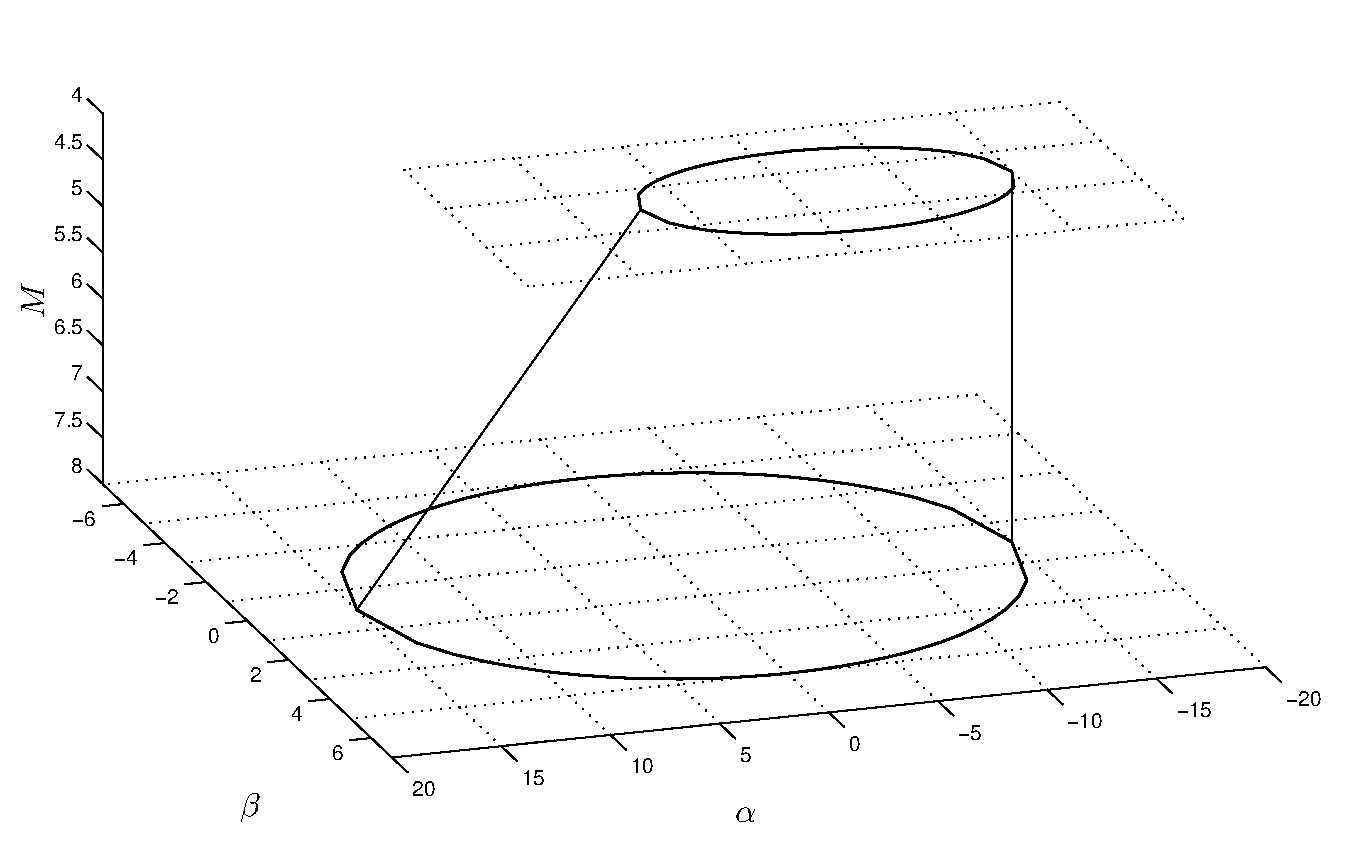
\includegraphics[width=4.0in]{\figurepath/unstart_cone_v2.eps}
    \caption{Ellipses defining region of started engine operation\label{fig:unstartcone}}
  \end{center}
\end{figure}

When unstart occurs the vehicle pitching moment is changed by a constant $\Delta C_{m_{0}}$, and slope $\Delta C_{m_{\alpha}}$ and the yawing moment by $\Delta C_{n_{0}}$, and slope $\Delta C_{n_{\beta}}$.

\begin{equation}
  C_{m}=C_{m_{\text{nom}}}+\Delta C_{m_{0}}+\Delta C_{m_{\alpha}}\alpha
\end{equation}
\begin{equation}
  C_{n}=C_{n_{\text{nom}}}+\Delta C_{n_{0}}+\Delta C_{n_{\beta}}\beta
\end{equation}

All engine force and moment contributions become zero, lift decreases by 20\%, and drag increases by 20\%.
Due to the time scale associated with the engine dynamics, engine unstart will essentially result in an instantaneous change in the plant dynamics.
The numerical values corresponding to the moment coefficient perturbations are examined more closely in Section~\ref{sec:unstartmodel}.
For the purposes of control design, it is assumed that pressure measurements at the combustor and inlet can be used to determine when unstart occurs\ \cite{wang.risk.2012}.

\begin{figure}[H]
  \fontsize{10pt}{10pt}\selectfont
  \begin{center}
    \psfrag{cont}[mc][mc][1.0]{\shortstack[c]{Baseline\\Controller}}
    \psfrag{adp}[mc][mc][1.0]{\shortstack[c]{Adaptive\\Controller}}
    \psfrag{unc}[tc][tc][1.0]{\fontsize{10pt}{10pt}\selectfont\bf\shortstack[c]{Unstart \\ model}}
    \psfrag{plant}[mc][mc][1.0]{Plant}
    \psfrag{r}[bc][bc][1.0]{$z_{\text{cmd}}$}
    \psfrag{un}[bc][bc][1.0]{$u_{\text{bl}}$}
    \psfrag{ua}[bc][bc][1.0]{$u_{\text{ad}}$}
    \psfrag{u}[bc][bc][1.0]{$u$}
    \psfrag{x}[bc][bc][1.0]{$x$}
    \psfrag{s}[mc][mc][1.0]{$+$}
    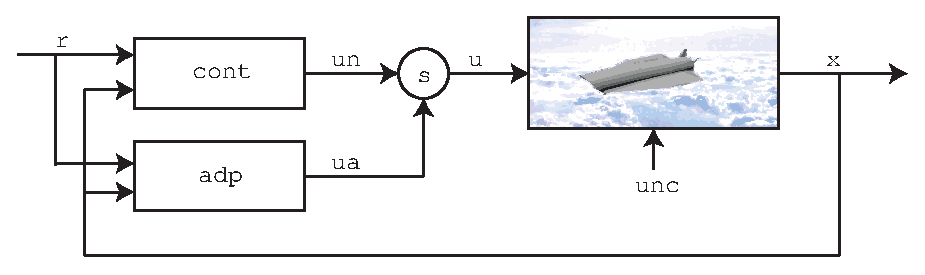
\includegraphics[width=5.5in]{\figurepath/long_term_goals_block.eps}
    \caption{Closed loop system block diagram with unstart model}
  \end{center}
\end{figure}

As future efforts improve the understanding of unstart, this information will be used to build a better unstart model, and guide the development of new novel adaptive strategies to cope with unstart.
